\documentclass[12pt,french,a4paper]{article}
\usepackage[utf8]{inputenc}
\usepackage[french]{babel}
\usepackage[T1]{fontenc}
\usepackage{fancyhdr}
\usepackage{lastpage}
\usepackage{fancybox}
\usepackage{graphicx}
\usepackage{appendix}
\usepackage[left=3cm,right=1cm,top=3cm,bottom=2cm]{geometry}
\geometry{a4paper}
\setlength{\parindent}{0pt}
\usepackage{listings}
\usepackage{color}
\usepackage[table]{xcolor}
\usepackage{array}
\usepackage{listings}
\usepackage{hyperref}
\usepackage{caption}
\usepackage{lastpage}
\pagestyle{fancy}

\definecolor{darkWhite}{rgb}{0.94,0.94,0.94}

\lstset{
  aboveskip=3mm,
  belowskip=-2mm,
  backgroundcolor=\color{darkWhite},
  basicstyle=\footnotesize,
  breakatwhitespace=false,
  breaklines=true,
  captionpos=b,
  commentstyle=\color{red},
  deletekeywords={...},
  escapeinside={\%*}{*)},
  extendedchars=true,
  framexleftmargin=16pt,
  framextopmargin=3pt,
  framexbottommargin=6pt,
  frame=tb,
  keepspaces=true,
  keywordstyle=\color{blue},
  language=C,
  literate=
  {²}{{\textsuperscript{2}}}1
  {⁴}{{\textsuperscript{4}}}1
  {⁶}{{\textsuperscript{6}}}1
  {⁸}{{\textsuperscript{8}}}1
  {€}{{\euro{}}}1
  {é}{{\'e}}1
  {è}{{\`{e}}}1
  {ê}{{\^{e}}}1
  {ë}{{\¨{e}}}1
  {É}{{\'{E}}}1
  {Ê}{{\^{E}}}1
  {û}{{\^{u}}}1
  {ù}{{\`{u}}}1
  {â}{{\^{a}}}1
  {à}{{\`{a}}}1
  {á}{{\'{a}}}1
  {ã}{{\~{a}}}1
  {Á}{{\'{A}}}1
  {Â}{{\^{A}}}1
  {Ã}{{\~{A}}}1
  {ç}{{\c{c}}}1
  {Ç}{{\c{C}}}1
  {õ}{{\~{o}}}1
  {ó}{{\'{o}}}1
  {ô}{{\^{o}}}1
  {Õ}{{\~{O}}}1
  {Ó}{{\'{O}}}1
  {Ô}{{\^{O}}}1
  {î}{{\^{i}}}1
  {Î}{{\^{I}}}1
  {í}{{\'{i}}}1
  {Í}{{\~{Í}}}1,
  morekeywords={*,...},
  numbers=left,
  numbersep=10pt,
  numberstyle=\tiny\color{black},
  rulecolor=\color{black},
  showspaces=false,
  showstringspaces=false,
  showtabs=false,
  stepnumber=1,
  stringstyle=\color{gray},
  tabsize=4,
  title=\lstname,
}

\fancyhead[L]{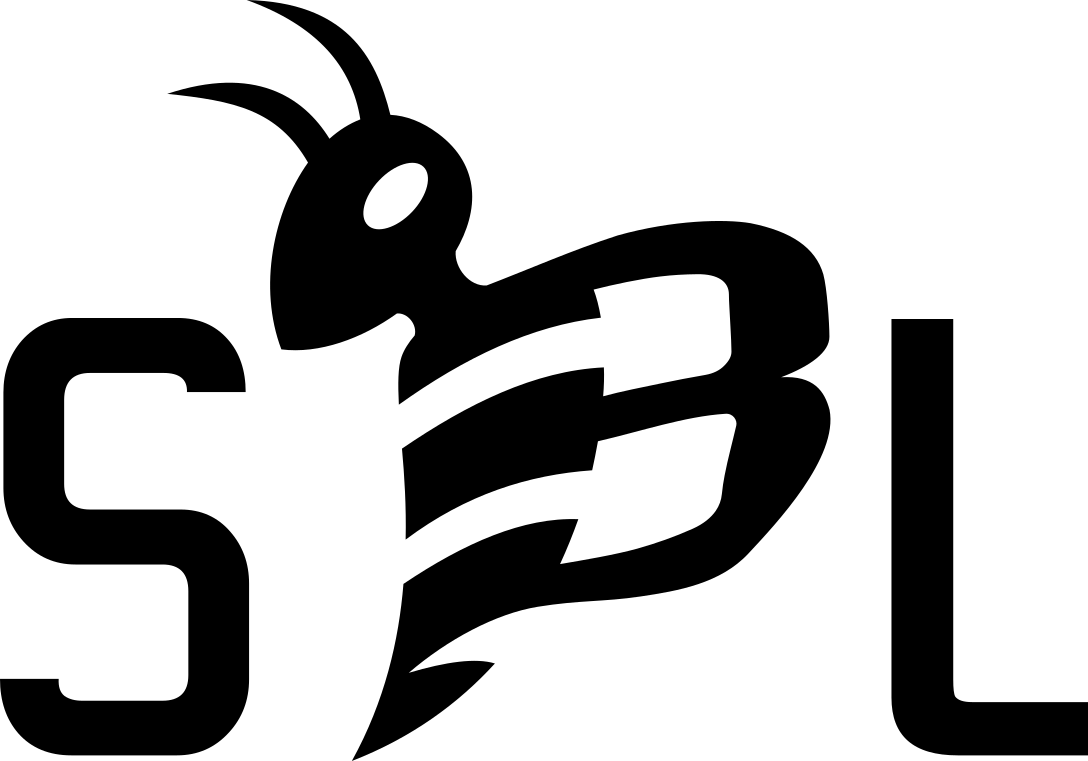
\includegraphics[width=1cm]{../../../logo/SBLlogo.png}}
\fancyhead[C]{Rapport d'activités mois de mai 2022 }
\fancyhead[R]{ 
\includegraphics[width=1.2cm]{../../../logo/IUTlogo.png}}
\fancyfoot[L]{\small Tom TUELEAU\normalsize}
\fancyfoot[C]{}
\fancyfoot[R]{\thepage/\pageref{LastPage}}

\lstset{
  basicstyle=\fontfamily{lmvtt}\selectfont\small,
  columns=fullflexible,
}

\title{
	\bigskip
 \centering
         
\includegraphics[width=4cm]{../../../logo/IUTlogo.png}  \hspace{7cm}
         
\includegraphics[width=4cm]{../../../logo/UMlogo.png}  \hspace{7cm}

	\LARGE{Rapport de stage}
	\\
	\LARGE{IBMM}
	\\
	\large{\textbf{Institut des Biomolécules Max Mousseron}}
	\\
	\large{Stagiaire :\textbf{Tom TUELEAU}}
	\\
	\large{Tuteur de stage :\textbf{Matthieu ROUSSET}}
	\\
	\large{Tuteur académique :\textbf{Sébastien DRUON}}
	\\
	\large{Durée du stage :\textbf{11 avril - 30 juin}}
	\\
	\large{RT2 :Promotion 2020-2022}
	\\
         
\includegraphics[width=4cm]{../../../logo/LIRMMlogo.png}  \hspace{7cm}
         \includegraphics[width=4cm]{../../../logo/IBMMlogo.jpg}  \hspace{7cm}
}
\author{
	\date{}
}

\begin{document}

\maketitle

\newpage
\section*{Remerciments}
J’adresse mes sincères remerciements aux personnes qui m’ont permis de réaliser ce stage.
Je souhaite remercier M. Matthieu Rousset, initiateur du projet SuperBeeLive,de m’avoir accepté au sein de son équipe.
Je souhaite également remercier Mme Olivia Serenelli-Pesin, qui a su m’encadrer et me guider. tout au long de ce stage
Je remercie également M. Sebastien Druon pour m’avoir conseillé et aiguillié quand j'ai rencontré des difficulté lors de mes mission.
Et enfin je remercie vivement toute l’équipe de pédagogique de Béziers, qui a su m'enseigner le savoir utile lors de ce stage.
\newpage

\section*{Resumer}
Ce stage c'est dérouler aux CNRS et à été encadrer par M. Matthieu Rousset chercheur à l'IBMM (Institut des Biomolécules Max Mousseron). \\
Si j'ai choisi ce stage c'est tout d'abords pour le sujet atypique reliant biologie, technologie et écologie. Ma seconde motivation était l'envie de découvrire plus en profondeur le monde de la recherche.\\ 
Ma mission principal lors de ce stage était de trouver un moyen de récolter les données de vibration et de températures et de les envoyer sur une basse de données afin qu'elle soit récuperable et visualisable sur un site web. Le site web et la basse de donnée n'était cependant pas compris dans ma mission. \\
Cette mission à été réaliser dans sont ensemble et ma permis d'acquerire des compétence en électronique et d'appliquer les connaisance acquise lors de mon DUT. 
\newpage
\section*{Remerciments}
\tableofcontents

\newpage
\section{Introduction}
\subsection{Mise en situation}
Mon stage prend place dans la continuité du projet SuperBeeLive. J'ai passer la majorité de mon stage au rucher, lieu ou sont entreposé une dizaine de ruches et ou la plus grand partie du projet SuperBeeLive prend place.
Nous étions plusieurs stagiaires installés à cet endroit. J'ai donc pu collaborer avec plusieurs d'entre eux notament sur la redaction de nos rapports. Comme vous pouvez le voir sur les figures \ref{intruch} et \ref{extruch}  nous étions installés dans un préfabriqué (climatisé et fibré) situé à côté des ruches.

\begin{center}	
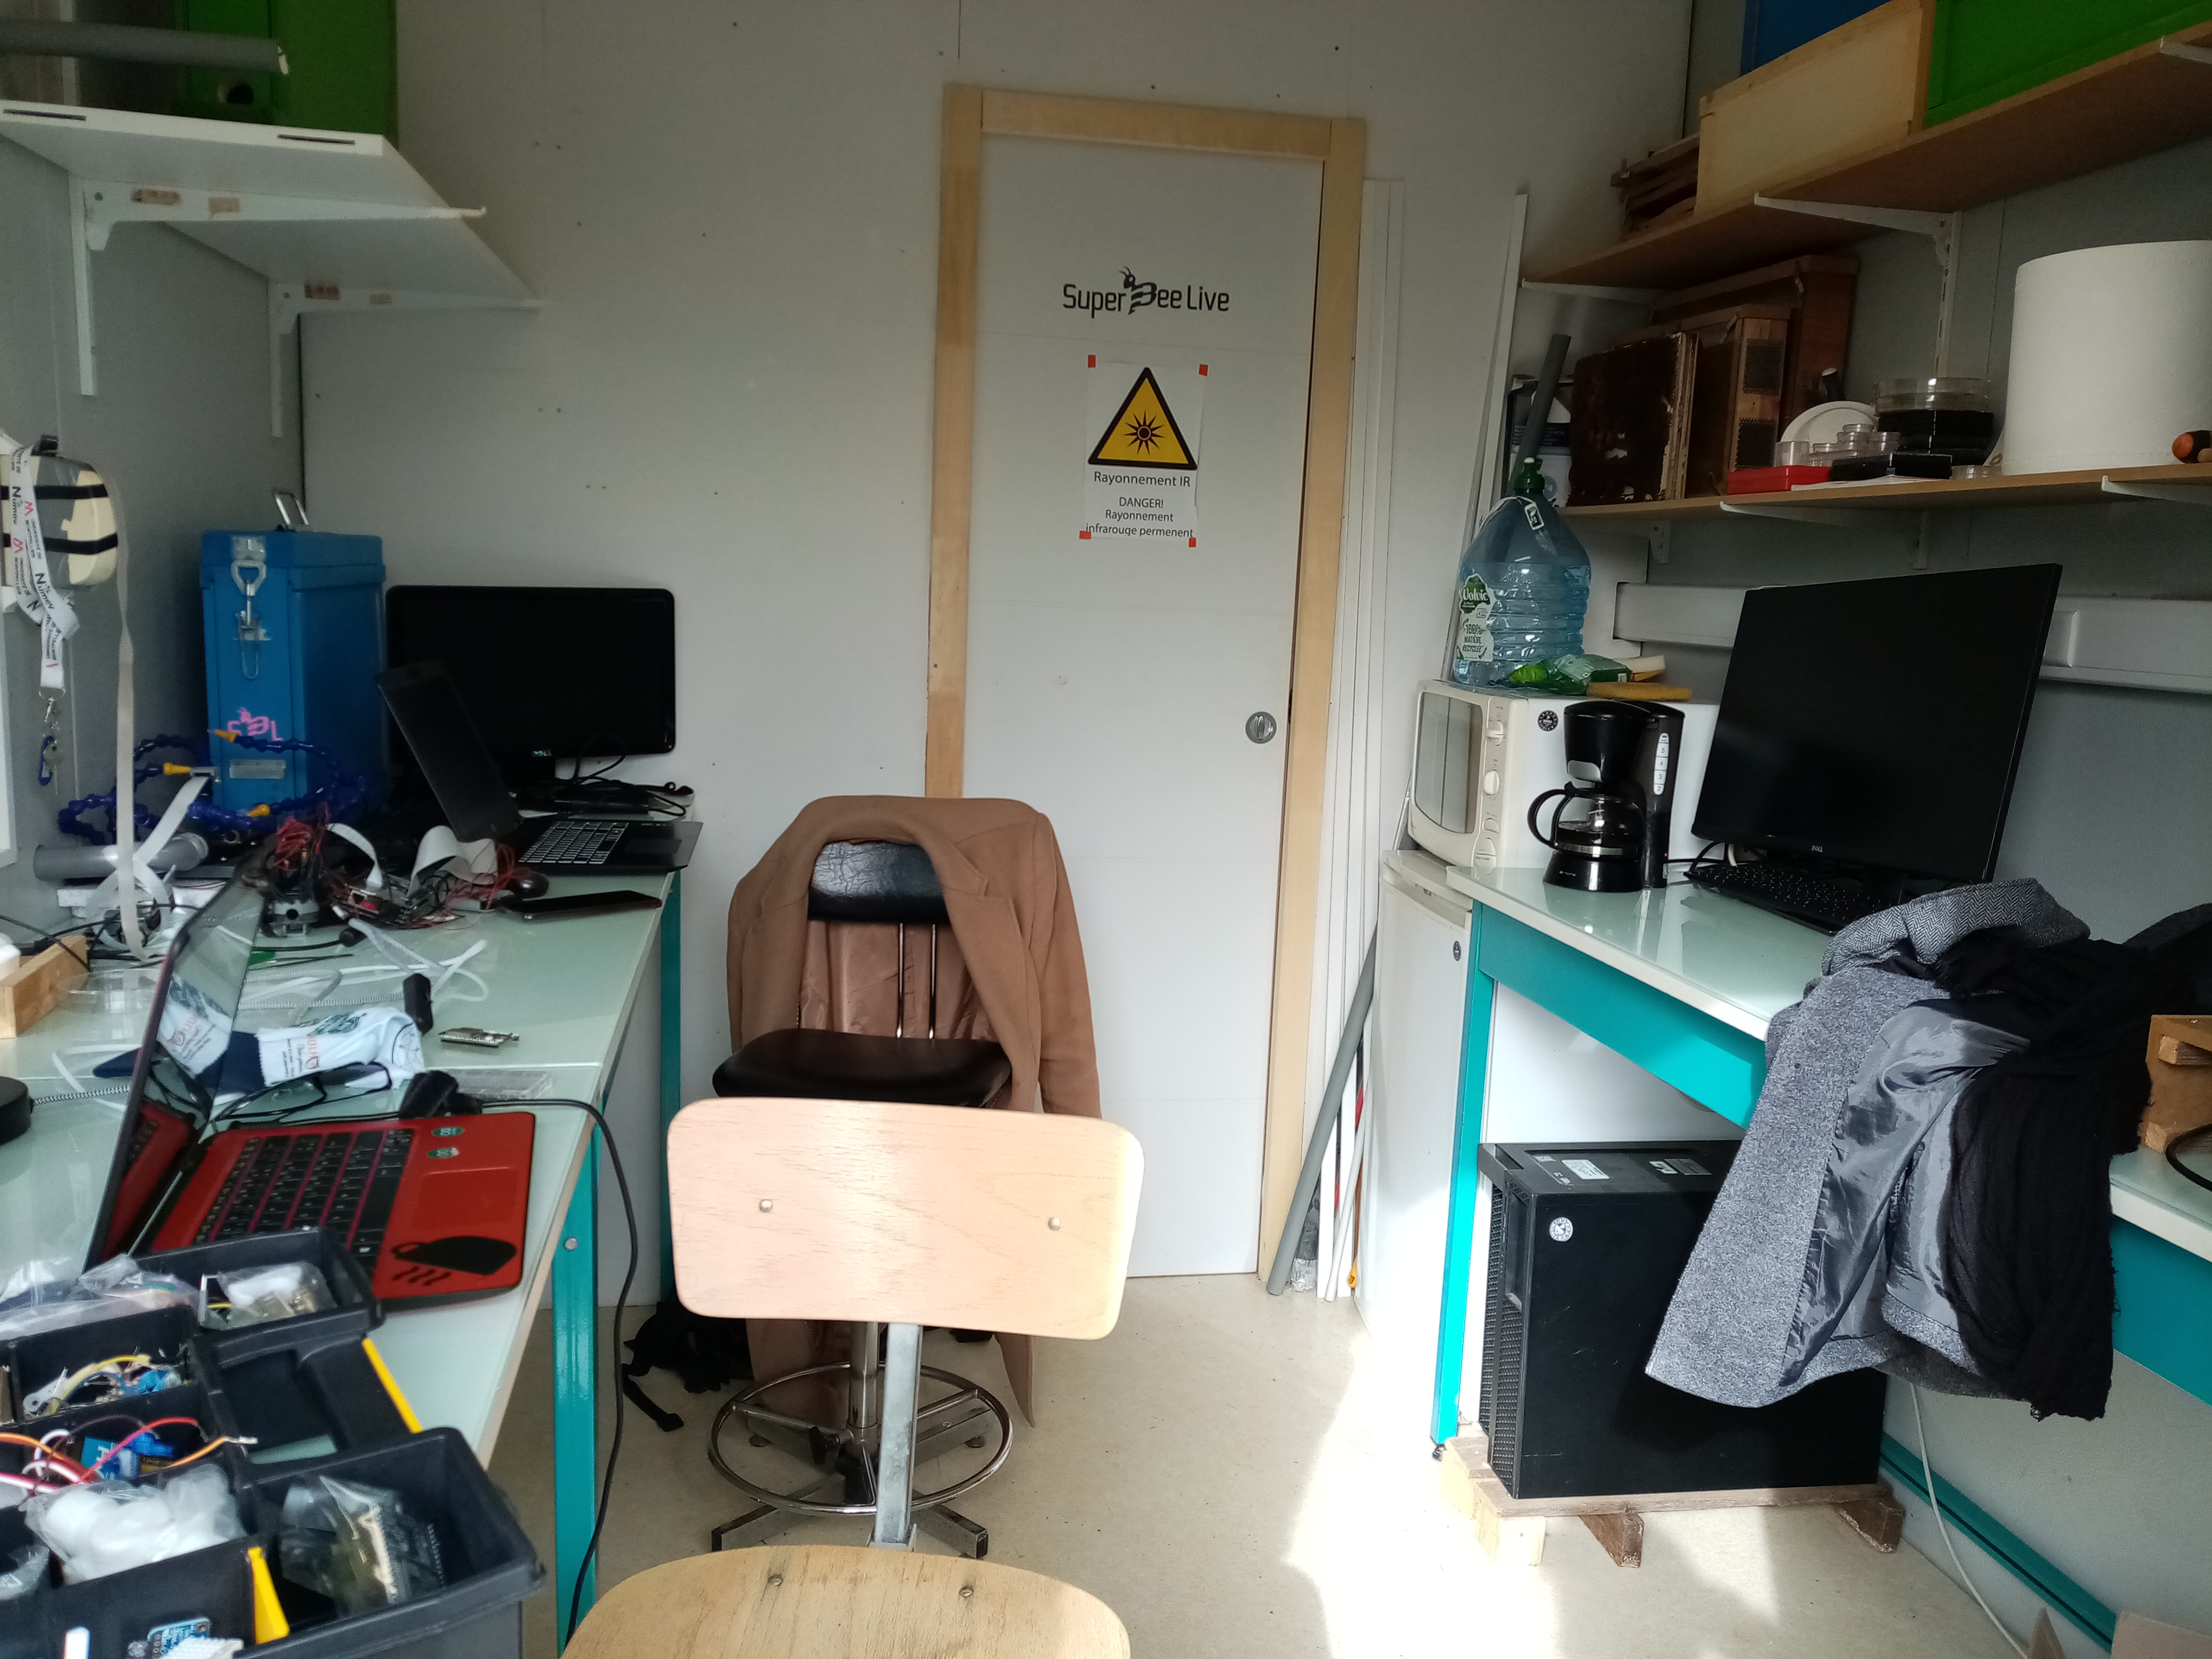
\includegraphics[scale=0.075]{../img/interieur_rucher.jpg}
\captionof{figure}{Intérieur du rucher}
\label{intruch}
\includegraphics[scale=0.075]{../img/exterieur_rucher.jpg}
\captionof{figure}{Extérieur du rucher}
\label{extruch}
\end{center}
\subsection{Sujet du stage}
Ce rapport fera état de l'activité réalisée lors du stage ainsi que l'état d'avancement des différentes missions confiées. Ma missions principale était la suivante : (Extrait de "sujets\_stage\_tom" de Mme Olivia SERENELLI-PESIN) 
\\
\\
\fbox{
	\begin{minipage}{17cm} 
	Nous avons besoin de mettre en place une première installation avec un micro-contrôleur et des capteurs dans la ruche afin de faire un "proof of concept" simple pour pouvoir afficher les données enregistrées sur le site internet où les vidéos des abeilles seront diffusées.\\
	\\
	Les données à enregistrer seront :\\
	— Température\\
	— Hygrométrie\\
	— Capteur de vibration fixé sur une gaufre de la ruche\\
	\\
	Elles devront être remontées en MQTT sur un serveur déjà mis en place.
	Le tout doit être opérationnel (fonctionnel et dans la ruche) avant le 15 Mai 2022.
	\\
	\end{minipage}
}
\\
\\
Je commencerai par vous décrire la manière dont je me suis organisé. Je décrirai dans une seconde partie aussi le réseau sur lequel j'ai travaillé, ainsi que les choix faits quand aux protocoles utilisés. Une troisième partie abordera les montages électroniques que j'ai découverts et testés lors de ce stage. Une dernier partie abordera la programmation des différents composants du système. Enfin, je conclurai en abordant les problèmes rencontrés ainsi que les améliorations possibles à mon travail.

\newpage
\section{Organisation}
Etant donné la durée assez courte du stage j'ai dû mettre en place des outils afin de pouvoir m'organiser et suivre l'avancée de mon activité tout au long du stage.
\\
J'ai cependant décidé d'adopter un nouvel outil afin d'organiser mon temps de travail. Je vous présenterai donc dans la prochaine partie le logiciel Notion, ainsi que mon utilisation de celui-ci.
\subsection{Notion}
Notion est une application web ayant plusieur utilités. Dans mon cas je m'en suis servi pour organiser le stage que ce soit en plannifient mes tâches, stockant mes notes ou en ayant une vision globale du travail à venir. Le plus important avec cet outils selon moi est la possibilités d'interconnecter chaque page entre elle. Cella permettant un re-croisement des données et une personnalisation poussée.  
\\
Chaque page que j'ai créée sur Notion possède une fonction précise. Je vais donc vous présenter chacune d'entre elles.

\subsubsection{Calendrier}
Comme son nom l'indique, la page calendrier répertorie chaque tâche ayant été effectuée sous la forme d'un calendrier. Cette page m'a permis de planifier et visualiser les dates butoires et à organiser mes semaines.    
\begin{center}	
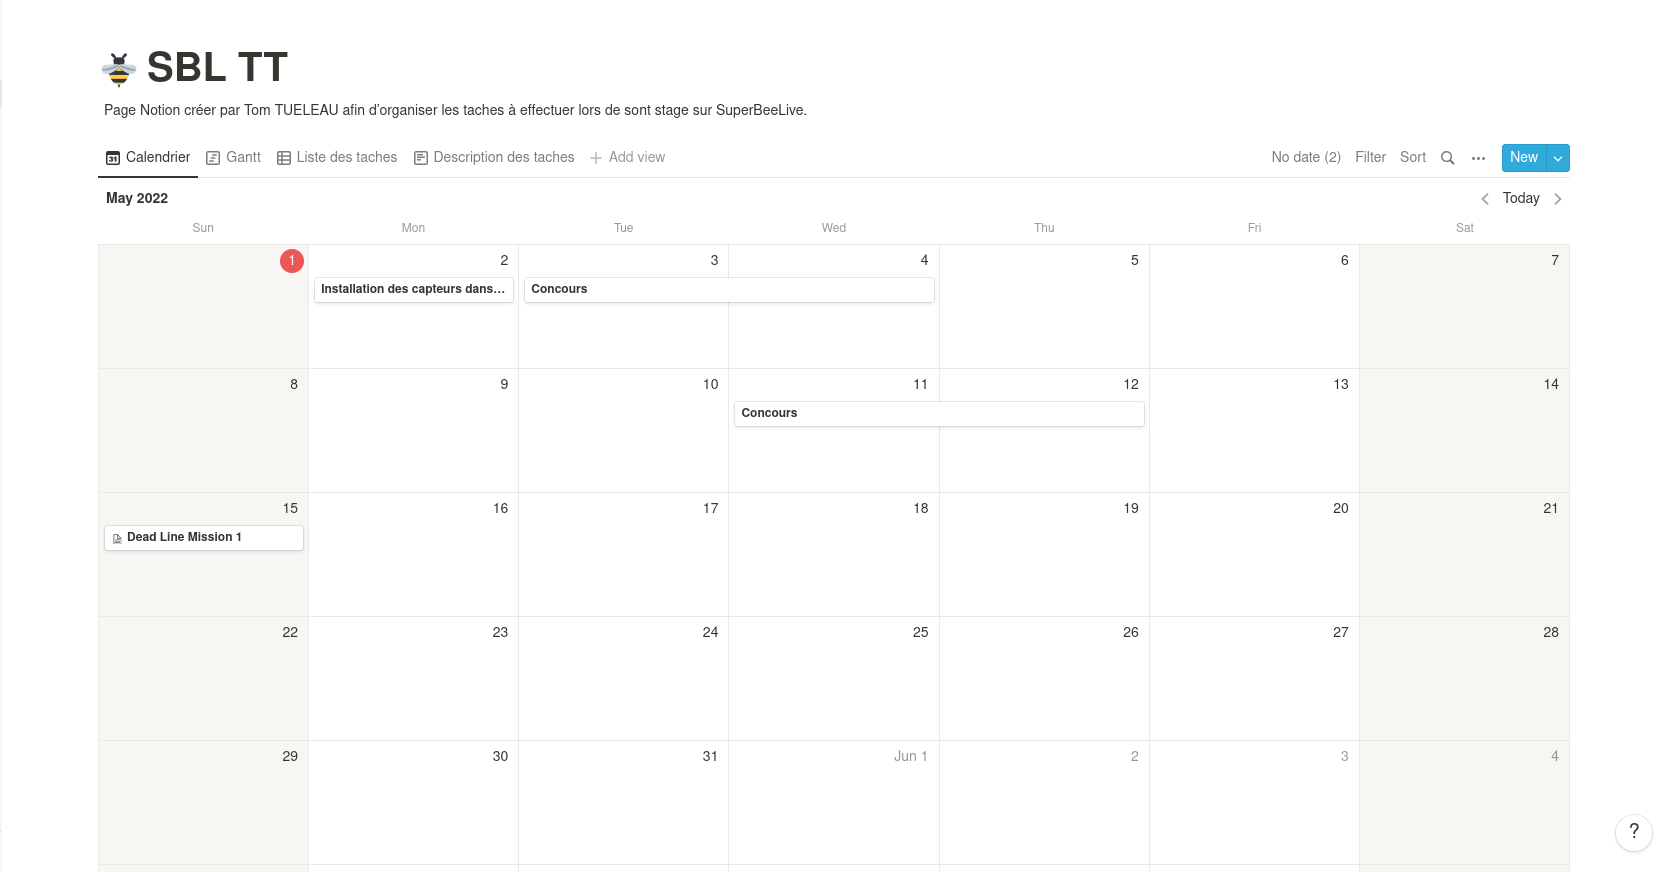
\includegraphics[scale=0.35]{../img/notioncalender.png}
\captionof{figure}{Calendrier}
\label{Calendrier}
\end{center}

\subsubsection{Liste des tâches}
La page "liste des tâches" regroupe toutes les tâches effectuées et à effectuer. J'attribue à ces tâches plusieurs caractéristiques. Tout d'abord à l'aide d'un système  étiquettes me permet de classer les tâches par ordre d'importance. Les différents niveaux sont "finis", "à faire", "en retard" et "urgente". La seconde caractéristique est la durée de réalisation attribuée cette tache. Ceci  couplé à la page "Calendrier" m'a permis de repérer les zones du projet où j'était en retard ou, encore les tâches m'ayant pris le plus de temps. Enfin une description dans laquelle je donne précisément les besoins de cette tâche. Chaque description comporte un texte résumant la tache, des photos et des liens utilisés pour réaliser la tâche.

\begin{center}	
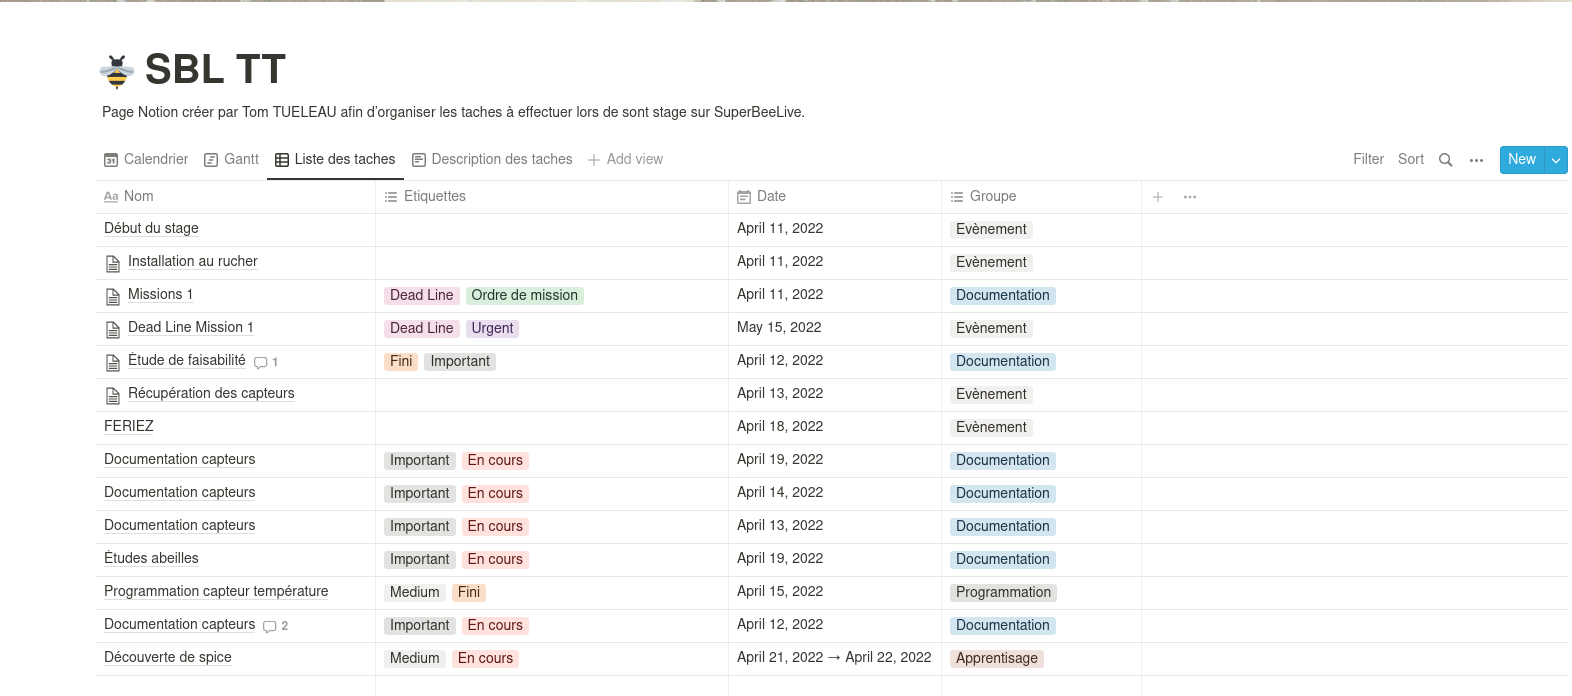
\includegraphics[scale=0.35]{../img/notionlistesdestaches.png}
\captionof{figure}{Liste des tâches}
\label{Liste des taches}
\end{center}
\newpage

\section{Topologie Réseau}
Comme nous pourons le voire dans cette partie le réseau peut étre décomposer en plusieur partie. Le rucher ou ce trouve SuperBeeLive et donc les caméras et appareil de messures. Et un serveur de stockage et de traitement au quel nous somme relier par deux fibre. 
\subsection{Ruche}
Dans le rucher on peut retrouver deux types d'équipements reliés au réseau. En premier lieu retrouvons 8 caméras ethernet délivrant un flux de 30 ips noir et blanc d'une résoltion de 1080 pixel. Le deuxième équipement est le micro-controleur récoltant les données des capteurs.  
\subsection{Interconnexion}
Comme dit précédement le système est composé de plusieurs éléments. Tout d'abord l'Arduino récolte les données et les envoie aux autres composantes. La température et l'humidité sont envoyés via MQTT vers le serveur tandis que les données du piezo sont envoyées via UDP. Une fois traité ces derniers sont aussi envoyés sur un topic MQTT.

\begin{center}
    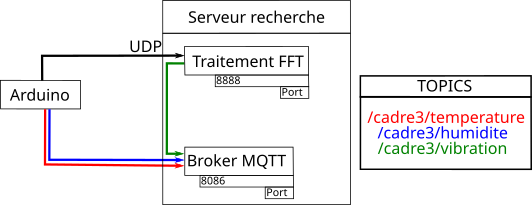
\includegraphics[scale=1]{../img/schemaNet.png}
	\captionof{figure}{Schema de concept du réseaux}
    \label{SN}
\end{center}

Afin d'envoyer les données du microcontroleur vers le serveur j'ai choisi le protocole MQTT, et ce pour deux raisons. La première est que le projet sera amené à évoluer et contiendra plusieurs capteurs récoltant la même donnée à des endroits differents de la ruche. Ainsi avec le systéme de topics, on pourra identifier facilement ces différents capteurs. La deuxième est que la solution envisagée pour le site web, et la base de données, est trés facilement couplable avec ce protocole. 

\subsubsection{Liaisons UDP}
Afin de transmetre les données du piezo au serveur, j'ai choisis d'effectuer une liaisons UDP. J'ai choisi ce protocole car la liaison n'as pas besoin d'accusé de réception. L'Arduino envoie donc sur le serveur les données du piezo.
Elle seront ensuite traiter et renvoyer à la base de données. 
Le traitement aurait pu ce faire sur l'Arduino mais les calcule étant asser lourd j'ai préferer les délocaliser sur une machine plus performente. Ainsi le role du microcontroleur est uniquement de récolter et envoyer les données. 

\newpage
\section{Eléctronique}
Lors de ce stage j'ai eux la chance de pouvoire effectuer de l'électronique. Afin que vous puisier visualiser les différent montage, vous trouverez tout au long de cette partie des schémas fait sous fritzing et des schémas plus rigoureux effectuer à l'aide de Kicad. Je ceommencerait donc par vous présenter mes choix quant aux composant utiliser. Une deuxiéme partie abordera les montage réaliser afin d'amplifier le signal du piezo-électrique.
\subsection{Choix des composants}

Le but de cette section est d'énoncer les possibilités que j'ai trouvées en ce qui concerne les composants demander (Capteurs d'humiditer de température et de vibration et micro-controleur). Nous commencerons par voir les différentes possibilités pour le micro-contrôleur et le choix effectuer. Ensuite, j'évoquerais les modèles des capteurs d'hygrométrie et de température aux quels j'ai songé. Enfin, je reviendrais sur le cas du capteur de vibration et les probématiques que j'ai pu rencontrer à sont égare.

\subsubsection{Micro-controleur}

Afin de remplire la mission, le micro controleur doit pouvoir :\\
\\
	- Récolter les données des differents capteurs\\
	- Envoyer les données via MQTT\\
	- Mise en place rapide et facile\\
	\\
De ces trois critères, j'ai retenue deux solutions possibles. 
Tout d'abord un arduino muni d'un shield Ethernet pourrait nous permettre dans un premier temps d'avoir un système 
connecté à internet et simple à mettre en place.
Dans un second temps, j'ai pensé à un Esp32 qui permettrait de faire transiter les données en Wifi et qui est plus petit. 
Étant familiarisé avec les deux solutions je n'avais pas de préférence. J'ai cependant commencé à travailler sur l'arduino, car j'avais le matériel à disposition.

\subsubsection{Capteur de température et d'hygrométrie }
Pour répondre à ce besoin, j'ai opté pour un Si7021. J'ai fait ce choix, car le capteur était directement à disposition et que je l'avais déjà utilisé. Ces caractéristiques sont les suivantes :\\
\\
\begin{center}
    \begin{tabular}{|l|l|}
	\hline
	    \multicolumn{2}{|c|}{Température} \\
	\hline
	    Plage de valeur & Résolution \\
	\hline
	    -40C - 125C & 0,4C \\
	\hline
    \end{tabular}
\end{center}
\begin{center}
    \begin{tabular}{|l|l|}
	\hline
	    \multicolumn{2}{|c|}{Humidité} \\
	\hline
	    Plage de valeur & Résolution \\
	\hline
	    0\% - 80\% & 0,3\% \\
	\hline
    \end{tabular}
\end{center}

\subsubsection{Capteur de vibration}
Le capteur de vibration est la partie que je connais le moins du projet. J'ai pu trouvé deux solutions.\\
 Une première à l'aide d'un capteur piézo-électrique et une seconde avec un  microphone. Ces deux capteurs étant les seules possibilités que j'avais à ma disposition, 
 j'ai décidé de les utiliser afin de savoir si elles pouvaient répondre aux besoins du projet.\\
\\
 Les deux références sont :\\
- p37e pour le piézo-électrique\\
- INMP441 pour le microphone.\\

Afin de pouvoir mesurer avec plus de précision les vibrations émises par les abeilles, j'ai pris conseil auprès de M. Rousset qui m'a fourni différents articles sur le sujet.
Après une lecture de ces documents, je suis arrivé à une estimation de la plage de fréquence de communication des abeilles dans la ruche à [200Hz-1000Hz]. Je me base sur l'extrait d'un échange avec M. Rousset pour déduire cette plage de valeurs : \\ 
\\
\\

\fbox{
	\begin{minipage}{17cm} 
Les vibrations dans les matériaux qui sont probablement détectées par plusieurs organes/structures dans le corps de l’abeille. Par exemple l’organe subgénual (subgenual organ) localisé dans la patte est sensible aux vibrations entre 200 et 1000Hz.
	\end{minipage}

}

Etant donné le temps à ma disposition à ce moment, j'ai préféré me baser sur ce résultat pour la commande des piézo-électriques et d'éfectuer les premier test avec le capteur qui était disponible. 

\subsubsection{Capteur Piézo-Electrique}

Afin d'analyser les caractéristiques du capteur fournis, j'ai commencé par chercher des documents en rapport avec celui-ci. Les recherches n'ayant pas 
été très concluantes, je suis très vite passé à l'analyse du capteur. J'ai commencé par relier la sortie de celui-ci à un oscilloscope, ensuite je le fixe
sur la table avec du scotch, puis, j'effectue des coups plus ou moins forts à une distance constante de celui-ci. J'ai donc pu relever des tensions allant de 20mV à 680mV.
Étant donné que nous cherchons à étudier les mouvements des abeilles, il me semble plus logique de me baser sur les valeurs les plus petites. Celles-ci correspondant à un frottement de stylo.
Par la suite j'ai donc cherché comment effectuer une amplification du signal. Je suis très rapidement tombé sur des montages à amplificateur opérationnel (AOP). J'ai donc commencé
à les étudier et ai pu expérimenter plusieurs montages notamment un montage amplifieur non-inverseur dont vous pouvez voir les clichés ci-dessous.
\begin{center}	
	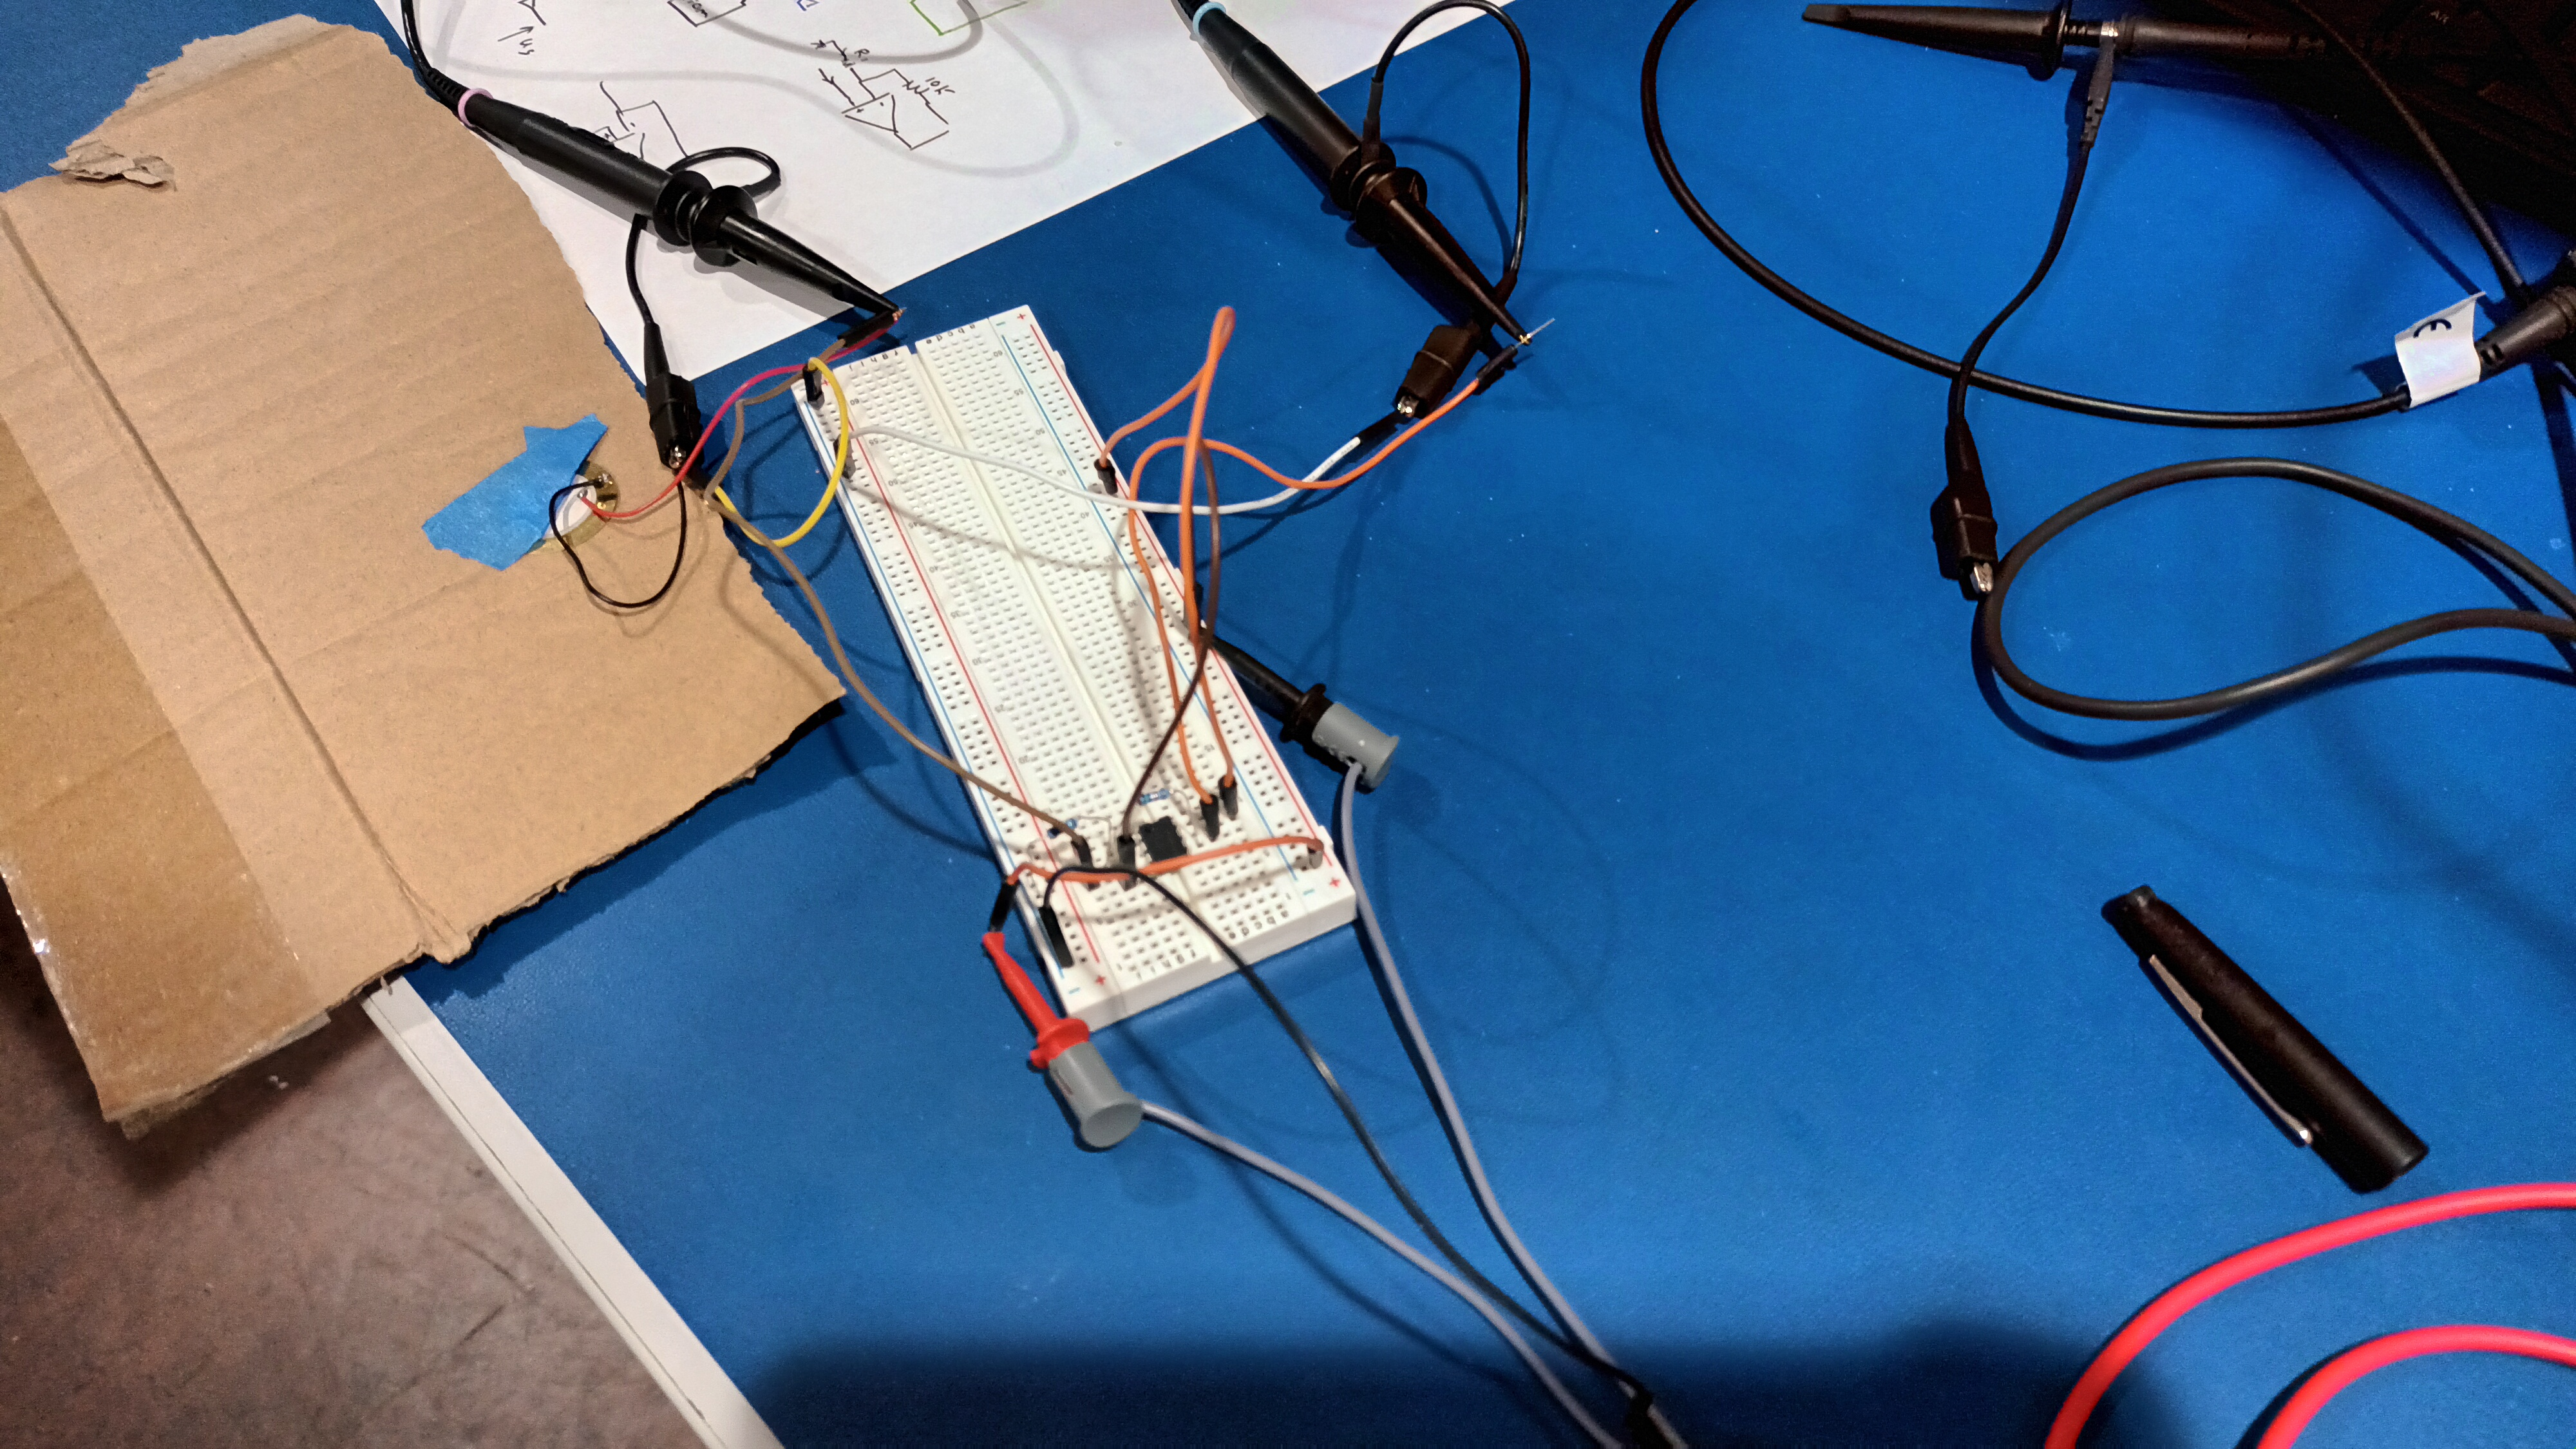
\includegraphics[scale=0.08]{../img/montage_piezo_aop.jpg}
	\captionof{figure}{Montage piezo AOP }
	\label{image3}
	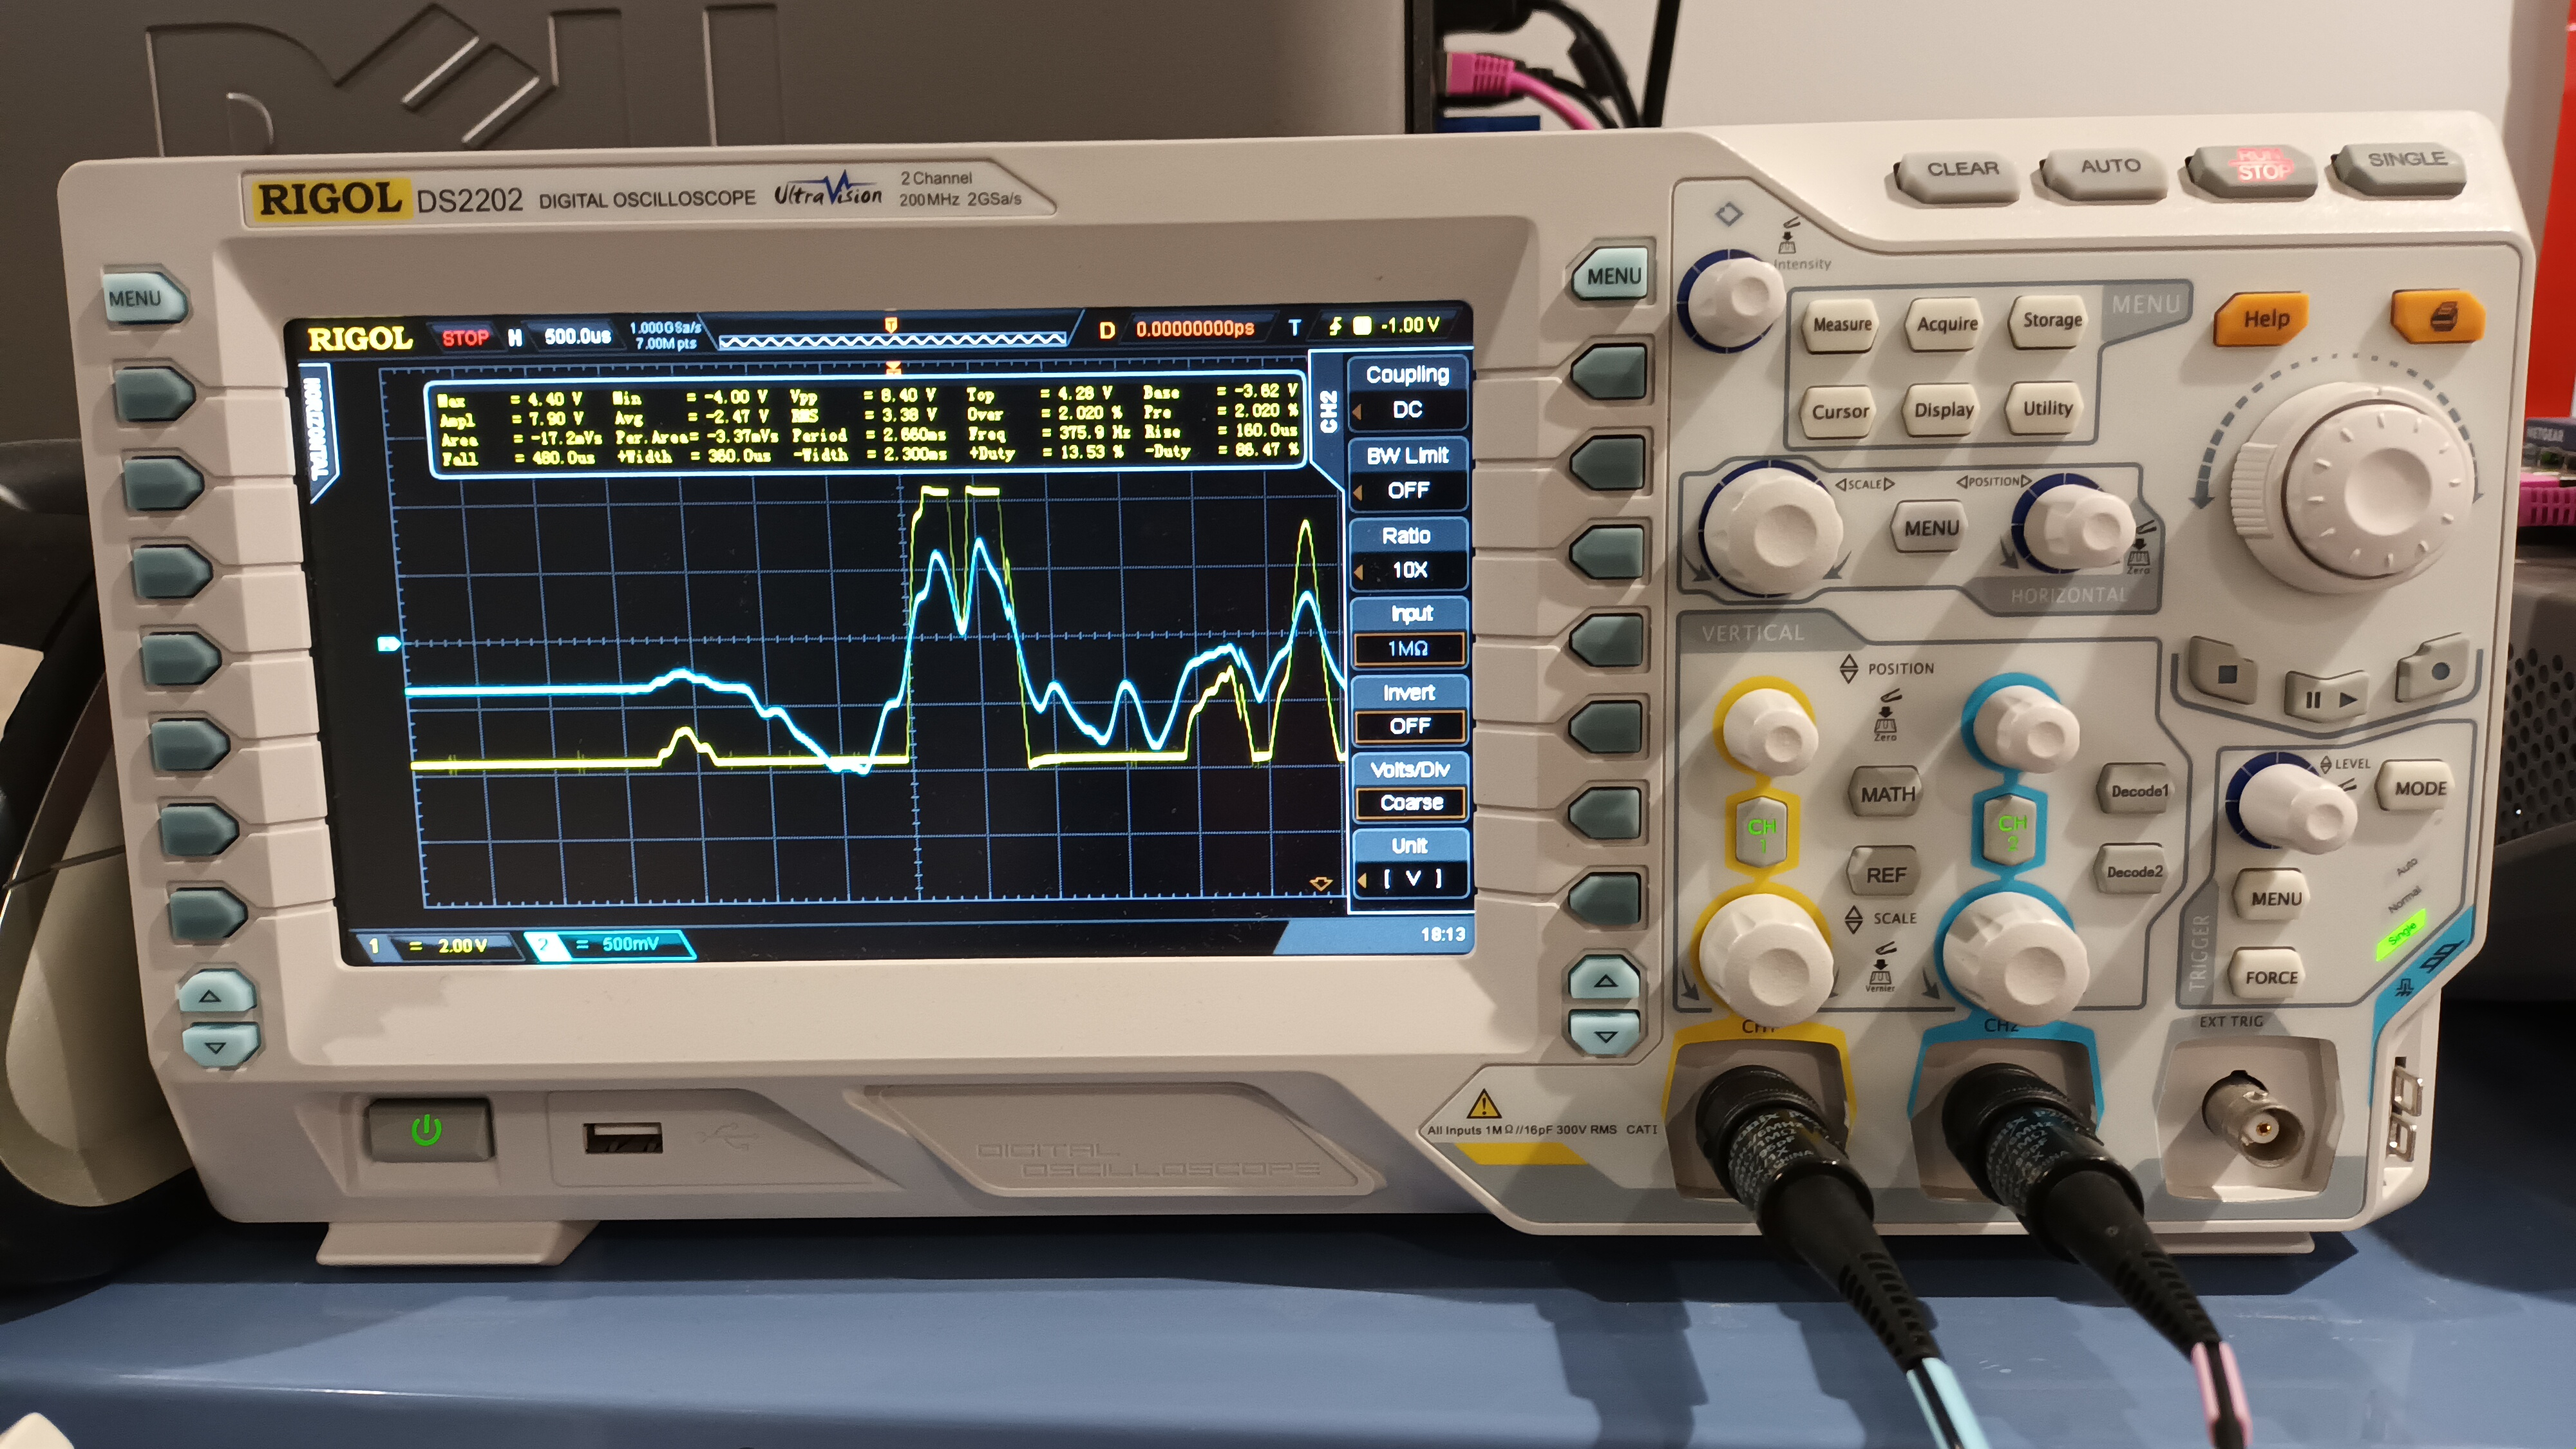
\includegraphics[scale=0.08]{../img/sortie_osciloscope.jpg}
	\captionof{figure}{Comparatif post et pré-amplification}
	\label{image4}
\end{center}

\newpage
\subsubsection{Amplificateur opérationel} 
Comme évoquer précedement j'ai eux à effectuer des montages avec des amplificateur opérationel (AOP). Le models que j'avais à ma disposition etait le LM342AN. Ce model prend la forme d'une puce à 14 broche et contenant en tout 4 AOP disctint. 

\subsection{Montages AOP}
Lors de ce stage j'ai du faire des recherches quand au dimensionnement d'un montage amplificateur. Ce besoin s'était fait ressentir quand je m'étais rendu compte que le signal émis par le piézo-électrique n'arrivait pas à être capté par l'Arduino.  Dans cette partie nous verrons tout d'abord le cheminement effectuer afin d'obtenire un montage fonctionnel. 

\subsubsection{Amplificateur de mesure}

Afin d'amplifier le signal mes encadrant mon coneiller de me renseigner sur les montages amplificateur de mesure. Ces montages sont très souvent utilisé afin d’amplifier le signal de sortie d’un capteur ayant une tension trop faible.
Il existe plusieurs montages amplificateur de mesures. Dans mon cas, j’ai expérimenter 2 d'entre eux. Un utilisant 2 AOP, visible figure \ref{2AOP}, et un second en utilisant 3, visible lui figure \ref{3AOP}. 

\begin{center}	
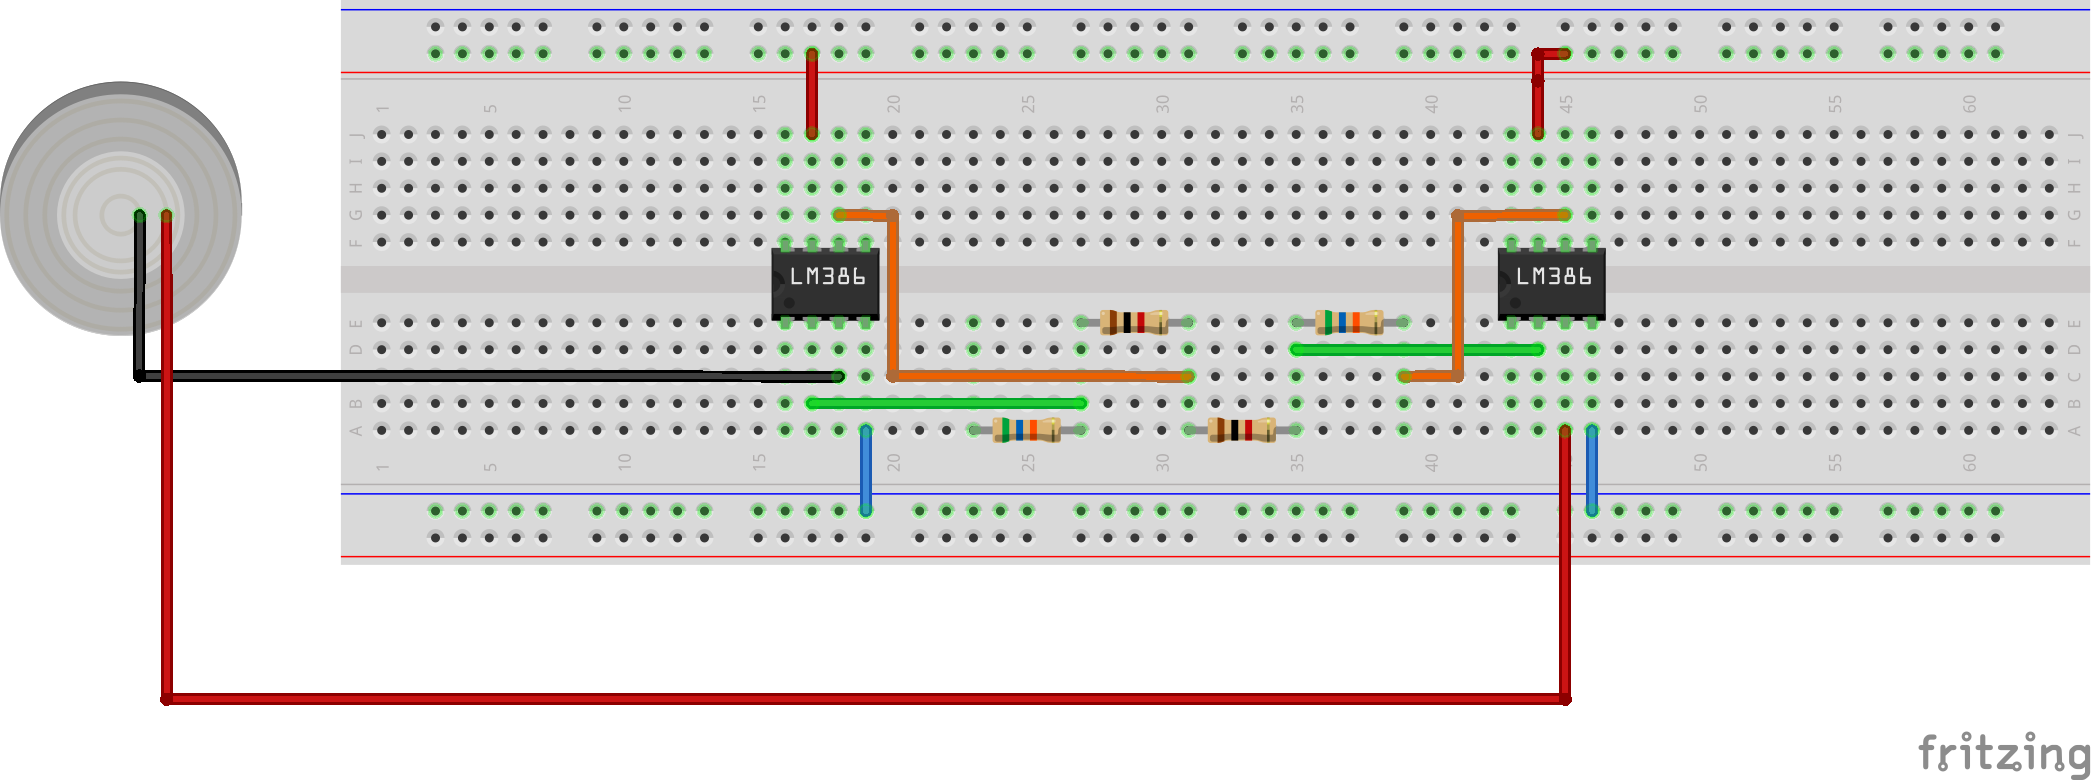
\includegraphics[scale=0.80]{../img/instrumentation2aop_bb.png}
\captionof{figure}{Montage 2 AOP sous Fritzing}
\label{2AOP}
\end{center}

\begin{center}	
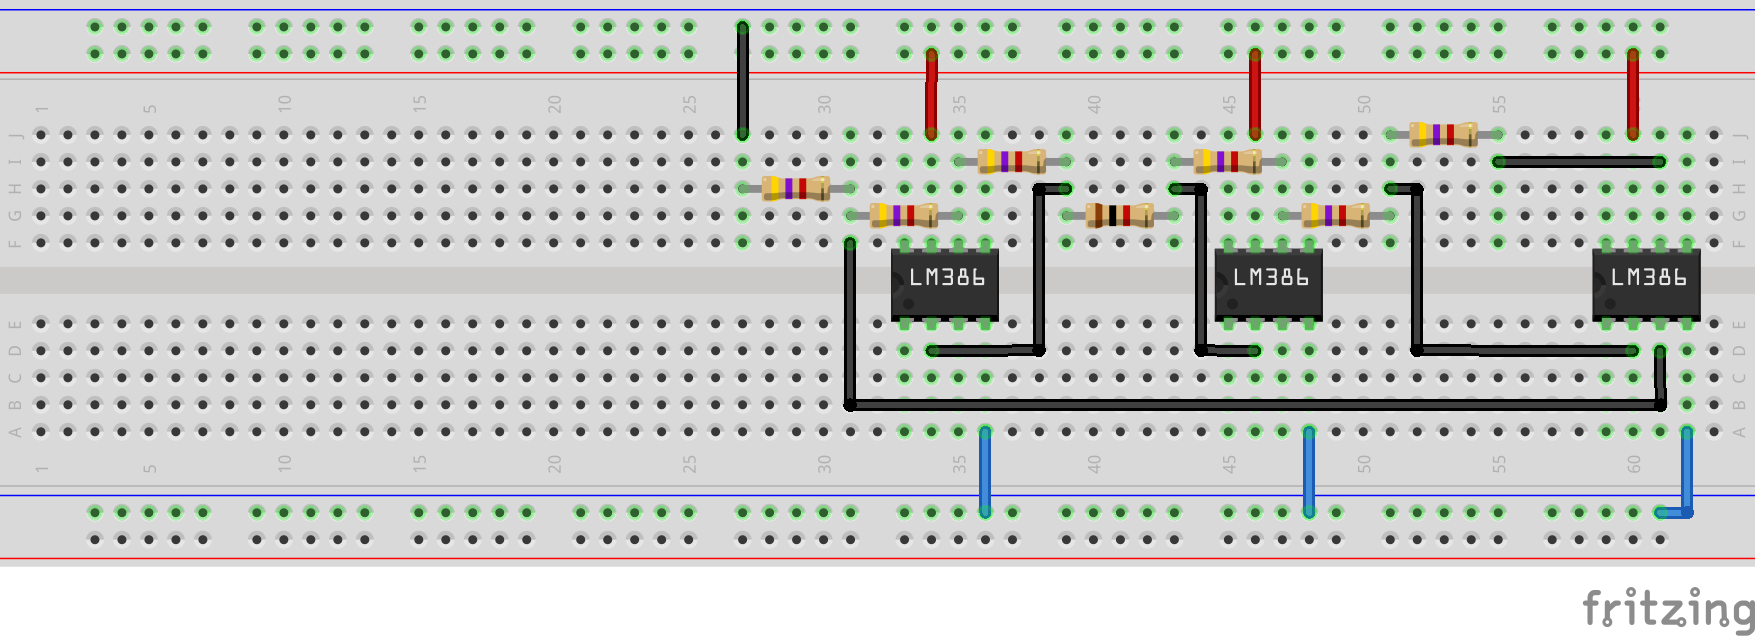
\includegraphics[scale=1]{../img/instrumentation3aop_bb.png}
\captionof{figure}{Montage 3 AOP sous Fritzing}
\label{3AOP}
\end{center}

Aprés avoir réussi à effectuer ce montage, j’ai pu remarquer que la sensibilité du capteur avait diminué. Ceci a eu pour effet de d’empêcher la visualisation d’impulsion créée lors de petits frottements.Ce probleme étant selon moi imputable à 2 élément. Tout d'abords une erreur de cablage de ma part, ou le model d'AOP que j'utilisait ne corespondait pas à cette utilisation. Etant données que nous cherchon surtout à amplifier les petit signaux, j’ai décidé de changer de montage.

\subsubsection{Montage actuel}
Le piezo-electrique utilisé jusqu’à maintenant était fourni avec un module. Celui-ci ne changeait rien au signal et pour cause, les composants sur lui n’étaient pas totalement connectés. Cependant, après avoir effectué des modifications sur celui-ci le signal m'a paru beaucoup plus net.
J’ai par la suite effecuté le montage visible figure \ref{MTGFINAL} et figure \ref{SMG}.
\\
\begin{center}	
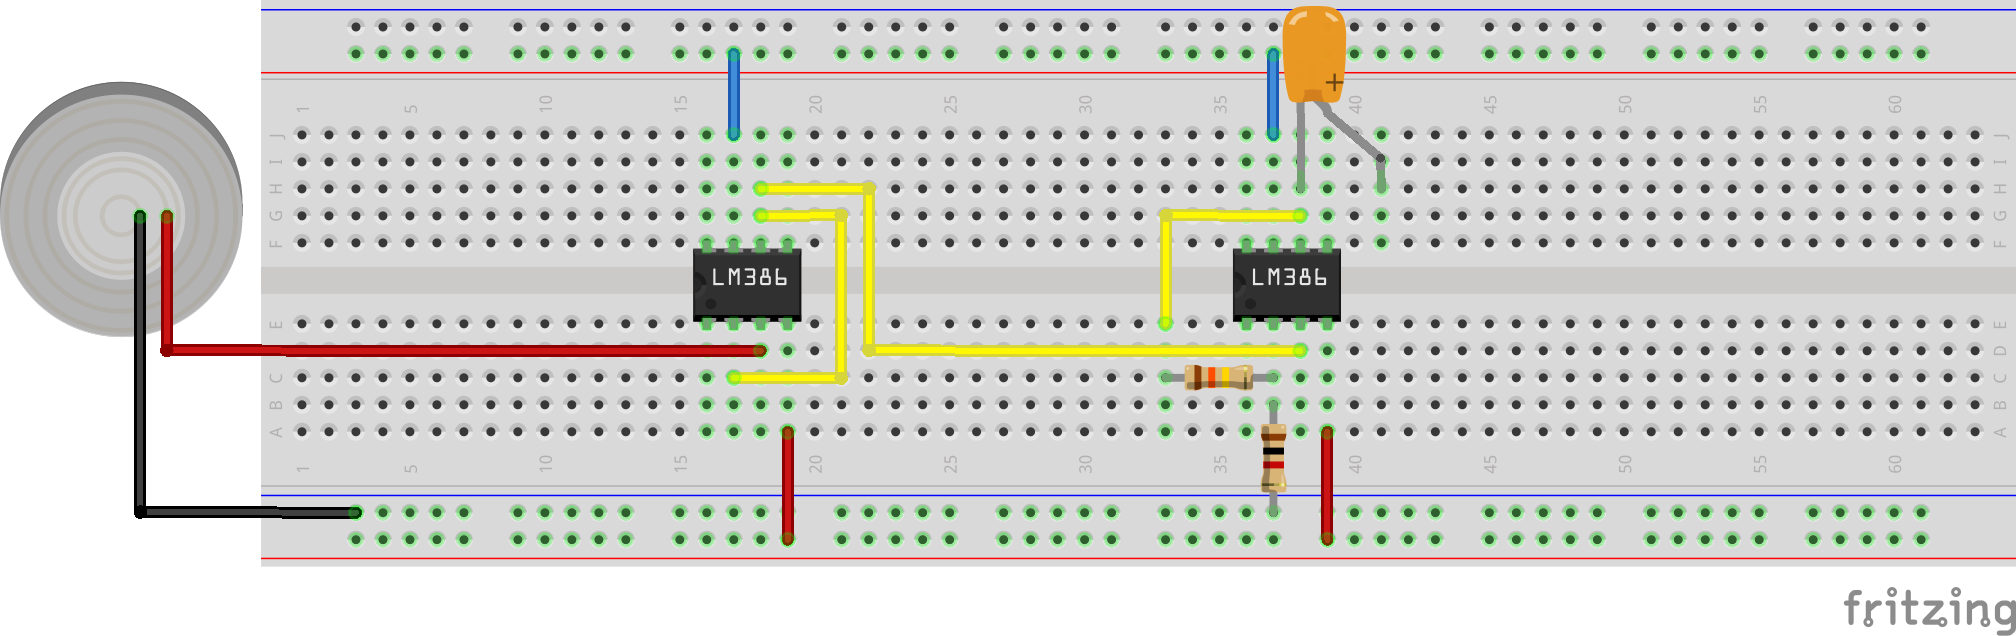
\includegraphics[scale=0.85]{../img/mtgfinal.png}
\captionof{figure}{Montage amplificateur}
\label{MTGFINAL}
\end{center}

\begin{center}
    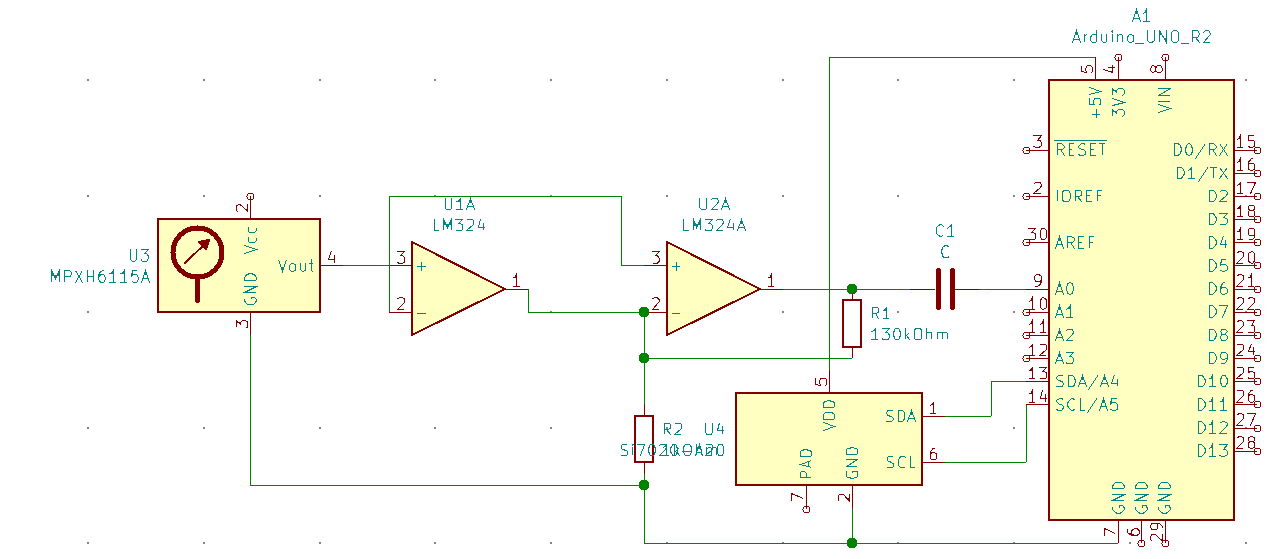
\includegraphics[scale=0.5]{../img/SMG.png}
    \captionof{figure}{Schéma montage final}
    \label{SMG}
\end{center}
Il est composé d’un suiveur et d’un amplificateur non-inverseur avec un coefficient multiplicateur de 130. C'est à dire que la tension de sortie sera 130 fois la tension d'entrée. Le coefficient est déterminer à partire de la formule suivante : \\ \\
\[
	Vs = Ve (1 + \frac{R1}{R2})
\]

Enfin, un condensateur se trouvant en sortie de circuit nous permet d’éliminer la composante continue ajoutée par les AOP à notre signal.


\subsubsection{Résultat}
Avec le montage vue précédemment nous obtenons plusieurs résultats probants.
Tout d'abord, nous pouvons voir figure \ref{VWOMVM} le signal en sortie du montage quand aucun évènement ne se produit.
Ensuite figure \ref{F}, nous pouvons voir la réaction après un léger frottement effectué avec un câble visible figure \ref{M}. 
On peut remarquer toujour sur la figure \ref{VMOMVM} un leger signal alternatif à 50Hz. Les test ayant été fait sur une breadboard il est possible quel récupére un signal émis par un appreil de mesure.

\begin{center}	
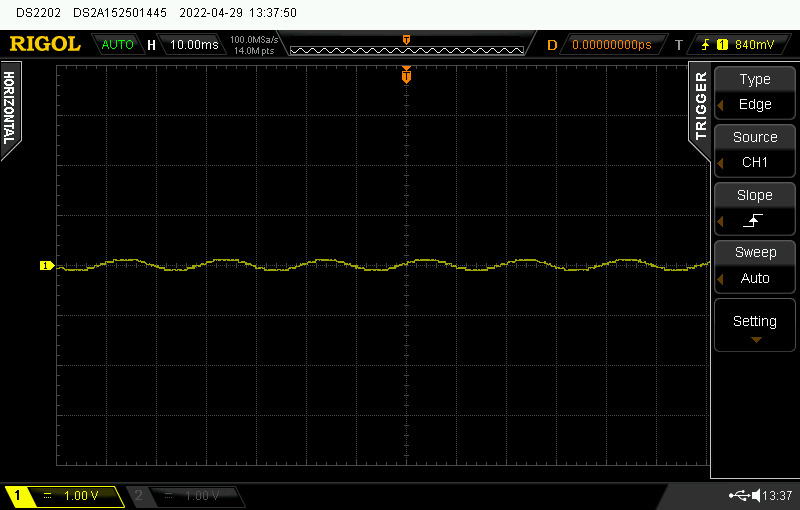
\includegraphics[scale=0.5]{../img/plat.jpg}
\captionof{figure}{Tension sans mouvement}
\label{VWOMVM}
\end{center}

\begin{center}	
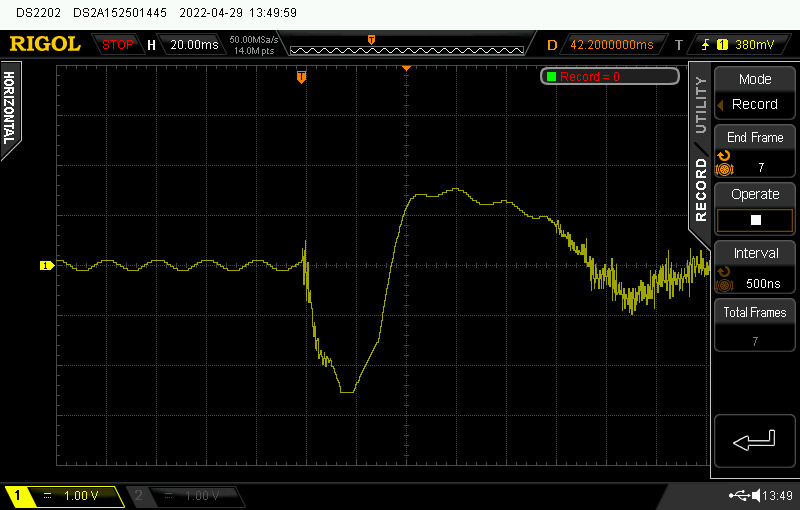
\includegraphics[scale=0.5]{../img/frotment.jpg}
\captionof{figure}{Tension lors d'un Frottement}
\label{F}
\end{center}

\begin{center}	
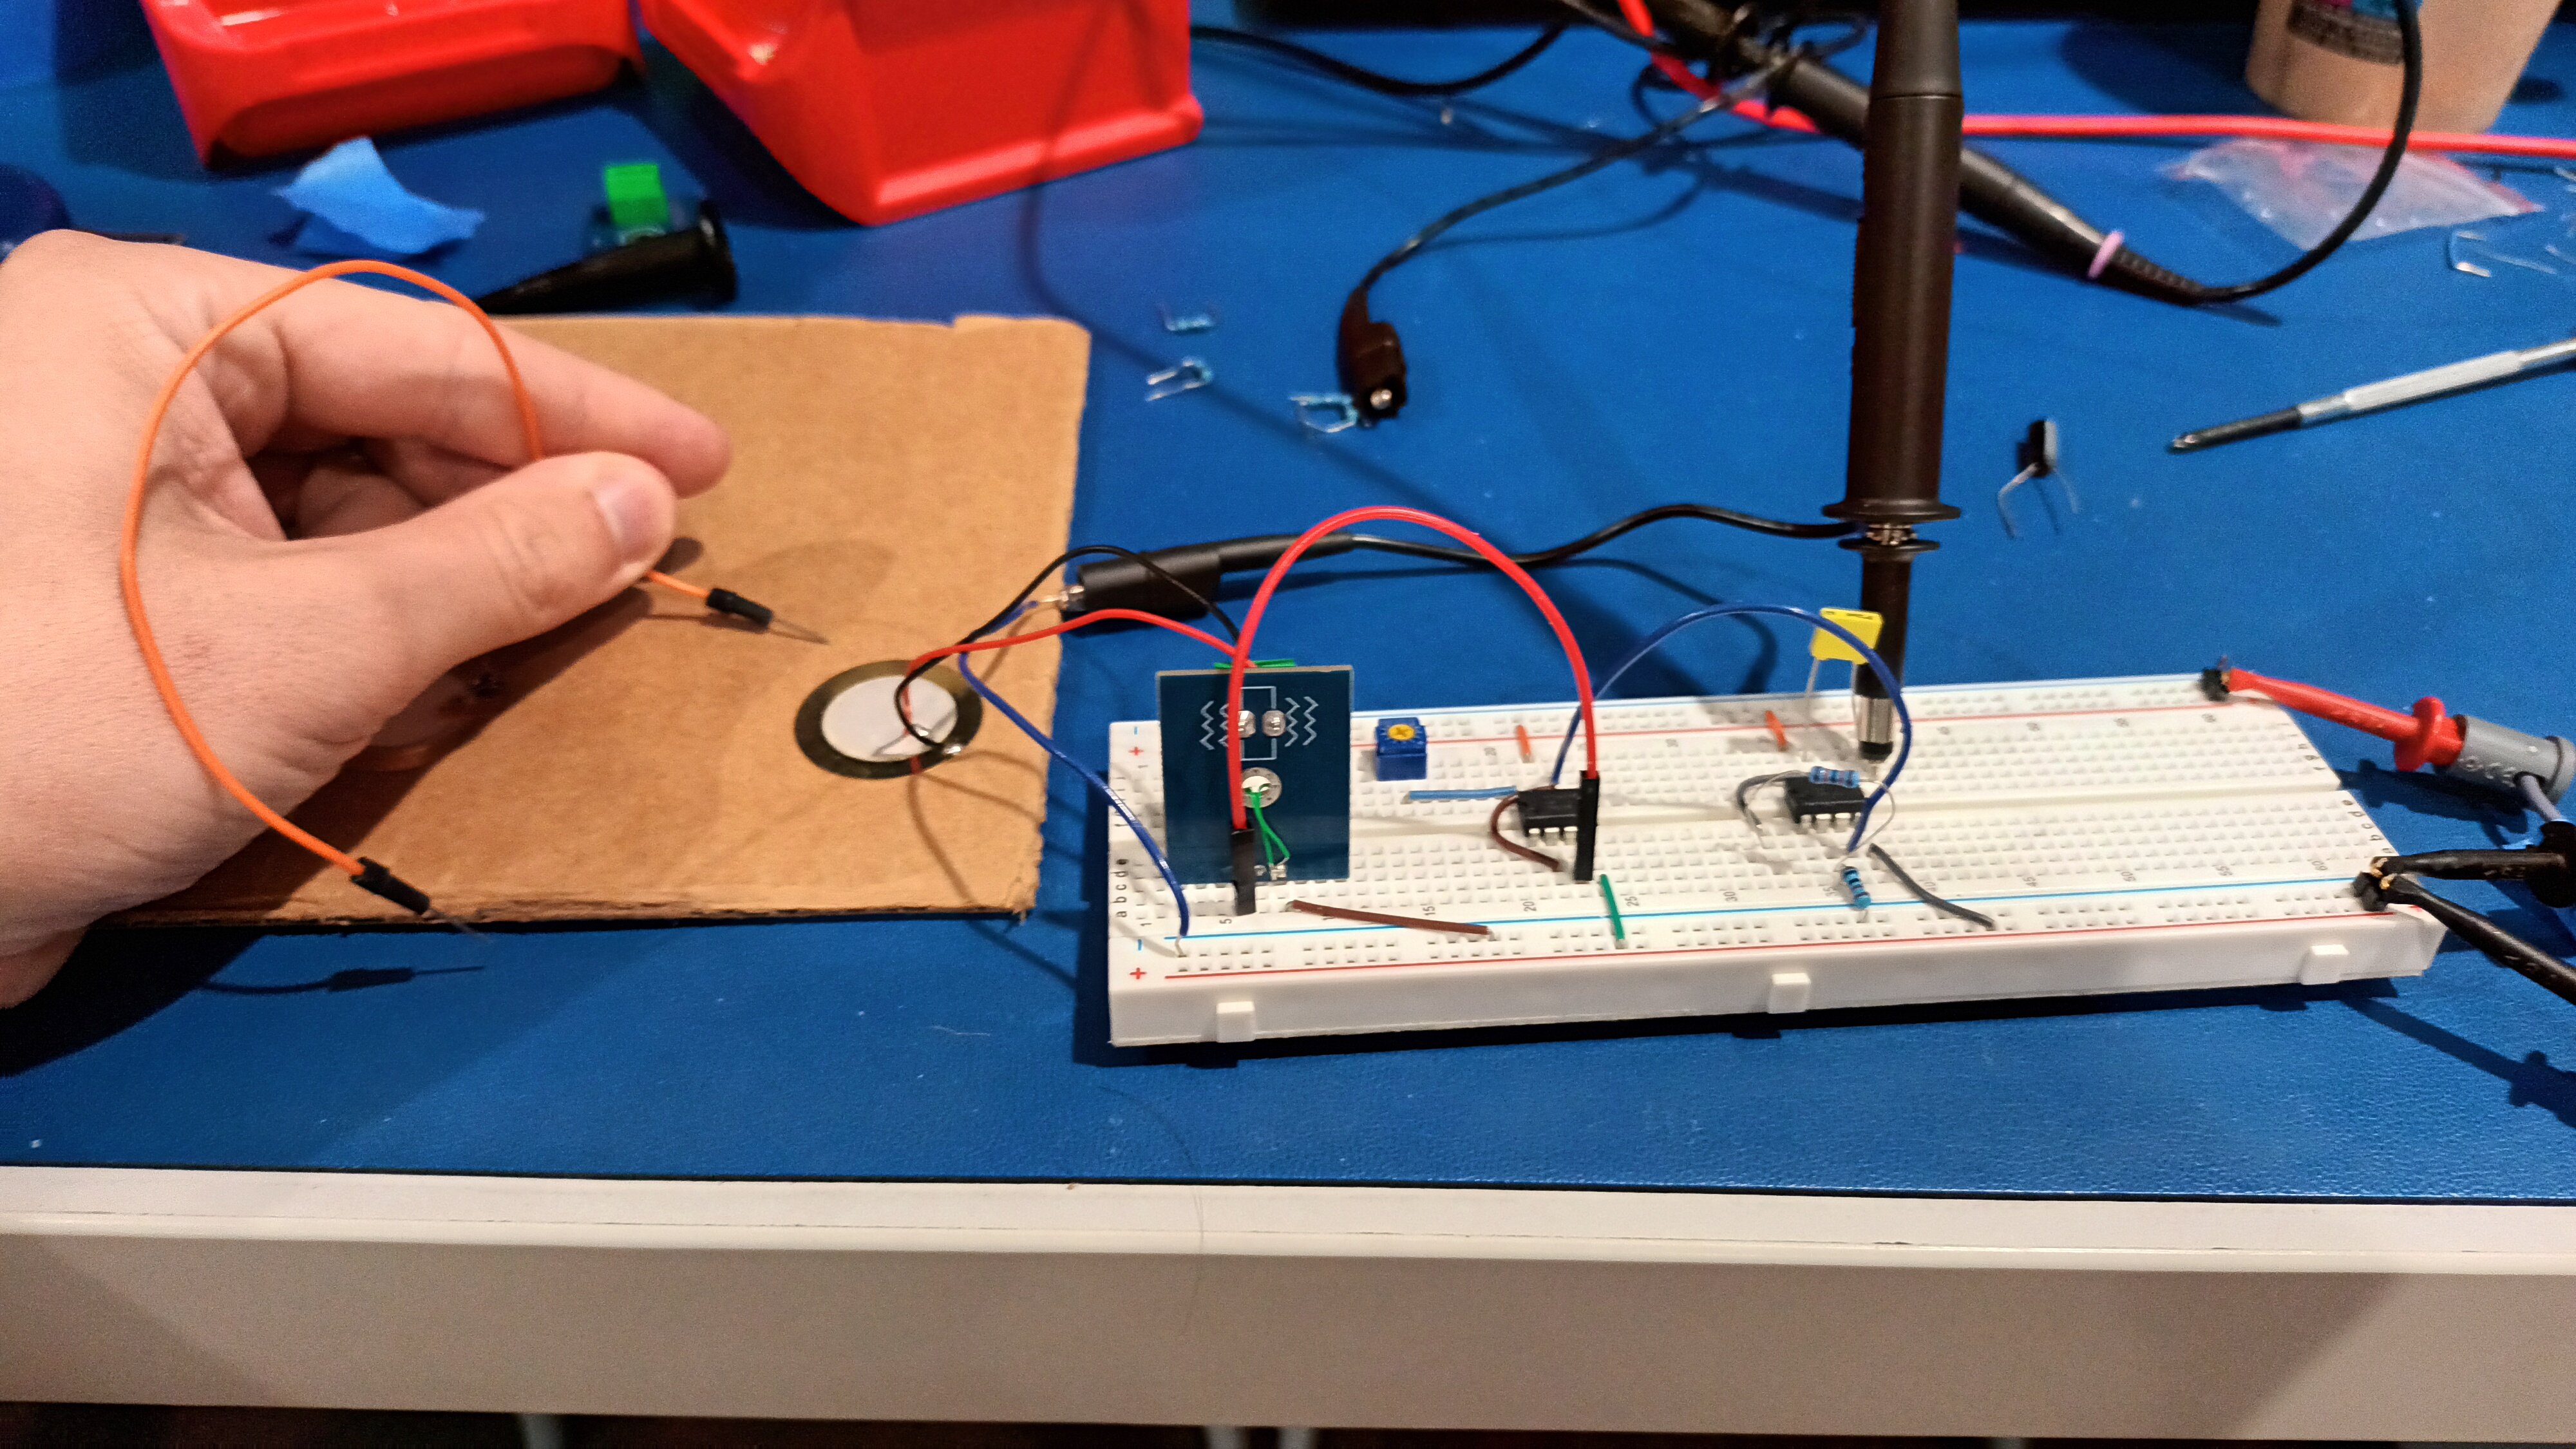
\includegraphics[scale=0.1]{../img/froty.jpg}
\captionof{figure}{Frottement}
\label{M}
\end{center}

\newpage
\section{Programmation}
Lors de ce stage j'ai été amener à faire plusieur programme. En \ref{Annexe} vous trouverez tout les codes réaliser. Je vais donc commencer par vous présenter la récolte des données et l'envoie de celle-ci. Dans une seconde partie je vous parlerait du traitement des données relatif au piezo. 

\subsection{Fonctionnement du programme}
Le progamme injecter dans l'arduino respect l'algorigramme suivant. 

\begin{center}	
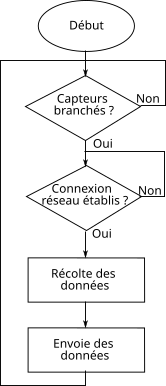
\includegraphics[scale=1]{../img/algorigrame.png}
\captionof{figure}{Algorigrame}
\label{M}
\end{center}
\subsection{Traitement}

Une fois le signal obtenu il fallait l'annalyser. J'avais dans un premier temps commencé à traiter les données directement sur l'Arduino en effectuant une transformé de Fourrier du signal. Cependant les capacités de calcul de l'Arduino étant limitées et ayant observé une certaine lenteur à effectuer cette opération j'ai décidé d'effectuer le systéme suivant. J'envoie les échantillons à un ordinateur distant qui effectuera le traitement et renvoie le résultat obtenu en MQTT.\\
J'ai donc par la suite écrit un programme utilisant la librairie "fftw". Celle-ci proposant de multiples fonctions bassées sur l'algorithme FFT (Fast Fourier Transform), permettant d'effectuer une transformée de Fourrier sur les signaux numérisés.\\
La raisons pour la quel j'ai decider de faire une transformer de fourier est tout simplement car l'objectif est d'annalyser en fréquence notre signal. Etant donner que cellui-ci n'est pas périodique j'ai du employer cette méthode afin de représenter sont spectre. Pour etre plus précis j'ai utiliser une transformer de fourier discret car nous somme sur un signal echantilloner. 
Le programme que j'ai écrits pour faire cella est disponible en annexe .  


\newpage
\section{Conclusion}
En conclusion, ce stage à été formateur pour moi tant dans l'approche que j'ai du mettre en place pour solutionner les probléme possé, que dans les différents domaines aborder. J'ai cependant rencontrer des difficulter sur certaine partie. En effet mes compétence en éléctronique ce limitant à des basique, j'ai abordées des composants complex comme l'amplificateur-opérationel avec certaine difficulter. J'ai cependant pu conter sur l'aide de mes encadrants afin de me diriger vers les bonnes sources d'information.


\newpage
\listoffigures

\newpage
\section*{Annexe}
\subsection*{Code}
\subsubsection*{Récolte et envoie des données}
\begin{scriptsize}
\begin{lstlisting}

//Libraries
// Communication serie on utilise :
// minicom -b 9600 -o -D /dev/ttyUC0


#include <SPI.h>
#include <PubSubClient.h>
#include <Ethernet.h>
#include <EthernetUdp.h>
#include <Adafruit_Si7021.h>
#define PORT_MQTT 1883
#define PORT_UDP 8888


void udpSendChar(char * data);
void gatherVibration(char * fdata, int nbEchantillon, int nbVirgule, double periodeEchantillonageMs);
void mqttSendHumTmp(int nbVirgule, Adafruit_Si7021 sensor);
void callback(char* topic, byte* payload, unsigned int length);
int beginEthSen();
int piezo = 0;
Adafruit_Si7021 sensor = Adafruit_Si7021();
String request ;
unsigned long refreshCounter  = 0;
byte mac [6] = {0x54, 0x34, 0x41, 0x30, 0x30, 0x31};
IPAddress ipMqtt(194, 199, 227, 239) ;
IPAddress ipUdp(10, 24, 4, 127) ;
EthernetUDP Udp;
EthernetClient ethclient; 
PubSubClient client(ipMqtt,PORT_MQTT,callback,ethclient); 

void setup() 
{
	Serial.begin(9600);
	if(!beginEthSen()){
		Serial.println("Erreur");
	}
	client.connect("arduino");
}
void loop() 
{
	char data[320];
	mqttSendHumTmp(2,sensor);
	gatherVibration(data,80,2,2);
	delay(1000);
}


// Lance tout les fonction. Ehternet, UDP, MQTT et le capteur. 
int beginEthSen()
{
	int error = 0;
	if (!sensor.begin()) 
	{
		Serial.println("Did not find Si7021 sensor!");
		error=1;
	}

	Serial.println(F("Initialize System"));
	Ethernet.begin(mac);

	while (!Ethernet.begin(mac)) 
	{
		Serial.println(F("failed. Retrying in 1 secondsi."));
		error=1;
	}

	pinMode(2, OUTPUT);
	pinMode(0, INPUT);
	Serial.print(F("IP Address: "));
	Serial.println(Ethernet.localIP());
	Udp.begin(PORT_UDP);
	if(error=1)
		return -1;

	return 0;
}


// Cette fonction recolte et envoie l'humiditer et la température en MQTT. nbVirgule permet de spécifier le nombre de valeur apres la virgule.
void mqttSendHumTmp(int nbVirgule,Adafruit_Si7021 sensor)
{

	double hum,temp;
	char Ctemp[2+nbVirgule];
	char Chum[2+nbVirgule];
	hum = sensor.readHumidity();
	temp = sensor.readTemperature();
	dtostrf(temp,2,nbVirgule,Ctemp);
	dtostrf(hum,2,nbVirgule,Chum);
  
  Serial.println("HUMIDITER ET TEMPERATURE");
	Serial.println(Chum);
	Serial.println(Ctemp);
	if(!client.publish("cadre3/temperature",Ctemp))
	{
		Serial.println("error");
	}
	if(!client.publish("cadre3/humidite",Chum))
	{
		Serial.println("error");
	}

}

void gatherVibration(char * fdata, int nbEchantillon, int nbVirgule, double periodeEchantillonageMs)
{
	// Afin d'avoire le nombre de caractere je fait le nombre de chiffre apres la virgule plus deux
	// qui represente mon premier digits et ma virgule.
	int nbChar = nbVirgule+2;
	char tmp[nbEchantillon][nbChar];
	char data2[nbEchantillon*nbChar];
	double centsValeurs[nbEchantillon];
	int i,y;
	for(i=0;i<nbEchantillon;i++){
		centsValeurs[i]=analogRead(piezo);
		centsValeurs[i]=(centsValeurs[i]*5)/1023;
		delay(periodeEchantillonageMs);
	}
	delay(2000);
	for(i=0;i<nbEchantillon;i++){
		dtostrf(centsValeurs[i],nbChar,nbVirgule,tmp[i]);
		for(y=0;y<nbChar;y++){
			data2[(nbChar*i)+y]=tmp[i][y];
		}	
	}
	Serial.println(data2);
	Udp.beginPacket(ipUdp,PORT_UDP);
	Udp.write(data2);
	Udp.endPacket();
}

void callback(char* topic, byte* payload, unsigned int length){

}
\end{lstlisting}
\end{scriptsize} 
\subsubsection*{Transformer de fourrier}
\begin{scriptsize}
\begin{lstlisting}

#include <stdio.h>
#include <complex.h>
#include <fftw3.h>
#include <stdlib.h>
#include <unistd.h>
#include <string.h>
#include <sys/types.h>
#include <sys/socket.h>
#include <arpa/inet.h>
#include <netinet/in.h>
//#include <arduinoUDP.h>

#define PORT	 8888
#define MAXLINE 2048

void traitementData(double * valeurs, char * charData, int taille, int nbChar);


int main (){

	printf("Début du programme. \n");
	int sockfd;
	char buffer[MAXLINE];
	struct sockaddr_in servaddr, cliaddr;
	double data[20];
	if ( (sockfd = socket(AF_INET, SOCK_DGRAM, 0)) < 0 ) {
		perror("Erreur lors de la creation de la socket");
		exit(EXIT_FAILURE);
	}

	memset(&servaddr, 0, sizeof(servaddr));
	memset(&cliaddr, 0, sizeof(cliaddr));

	servaddr.sin_family = AF_INET; 
	servaddr.sin_addr.s_addr = INADDR_ANY;
	servaddr.sin_port = htons(PORT);

	if ( bind(sockfd, (const struct sockaddr *)&servaddr,sizeof(servaddr)) < 0 )
	{
		perror("bind failed");
		exit(EXIT_FAILURE);
	}

	int len, n;

	len = sizeof(cliaddr); //len is value/result
	for(;;){
		n = recvfrom(sockfd, (char *)buffer, MAXLINE,MSG_WAITALL, ( struct sockaddr *) &cliaddr,&len);
		buffer[n] = '\0';
		printf("Client : %s\n", buffer);
		traitementData(data,buffer,20,4);
	}
	return 0;
}

void traitementData(double * valeurs, char * charData, int taille, int nbChar){
	int i,y;
	char tmp[4];
	printf("\n");
	for(i=0;i<taille;i++){
		for(y=0;y<nbChar;y++)
			tmp[y]=charData[(i*nbChar)+y];
		valeurs[i]=atof(tmp);
		printf("%f ",valeurs[i]);
	}
	printf("\n ");
}
\end{lstlisting}
\end{scriptsize} 
\end{document}
